\section{Migrations of Tracks into and out of the~Fiducial Region}\label{section:star_okr}
The procedure, described in this section, accounts for migrations of tracks into and out of the fiducial region, which originate from TPC resolution effects. The correction factor for such tracks, $f_\textrm{okr}(p_T, \eta)$ is defined as follows:
\begin{equation}
f_\textrm{okr}(p_\textrm{T}, \eta)=\frac{1-f_\textrm{okr}^-(p_\textrm{T}, \eta)}{1-f_{okr}^+(p_\textrm{T}, \eta)}
\end{equation}
where:
\begin{description}
	\item $f_\textrm{okr}^-(p_\textrm{T}, \eta)$ is the fraction of reconstructed tracks for which the corresponding primary particle is outside of the kinematic range of the measurement,
	\item $f_\textrm{okr}^+(p_\textrm{T}, \eta)$  is the fraction of primary particles for which the corresponding reconstructed track is outside of the kinematic range of the measurement.
\end{description}
The resulting residual migrations, shown in Fig.~\ref{fig:okr}, were estimated using MC. The main effect  was observed  at $|\eta| \sim 0.7$, where about $2-6\%$ reconstructed tracks were associated to primary particle outside the fiducial region.  

\begin{figure}[h!]
	\centering
	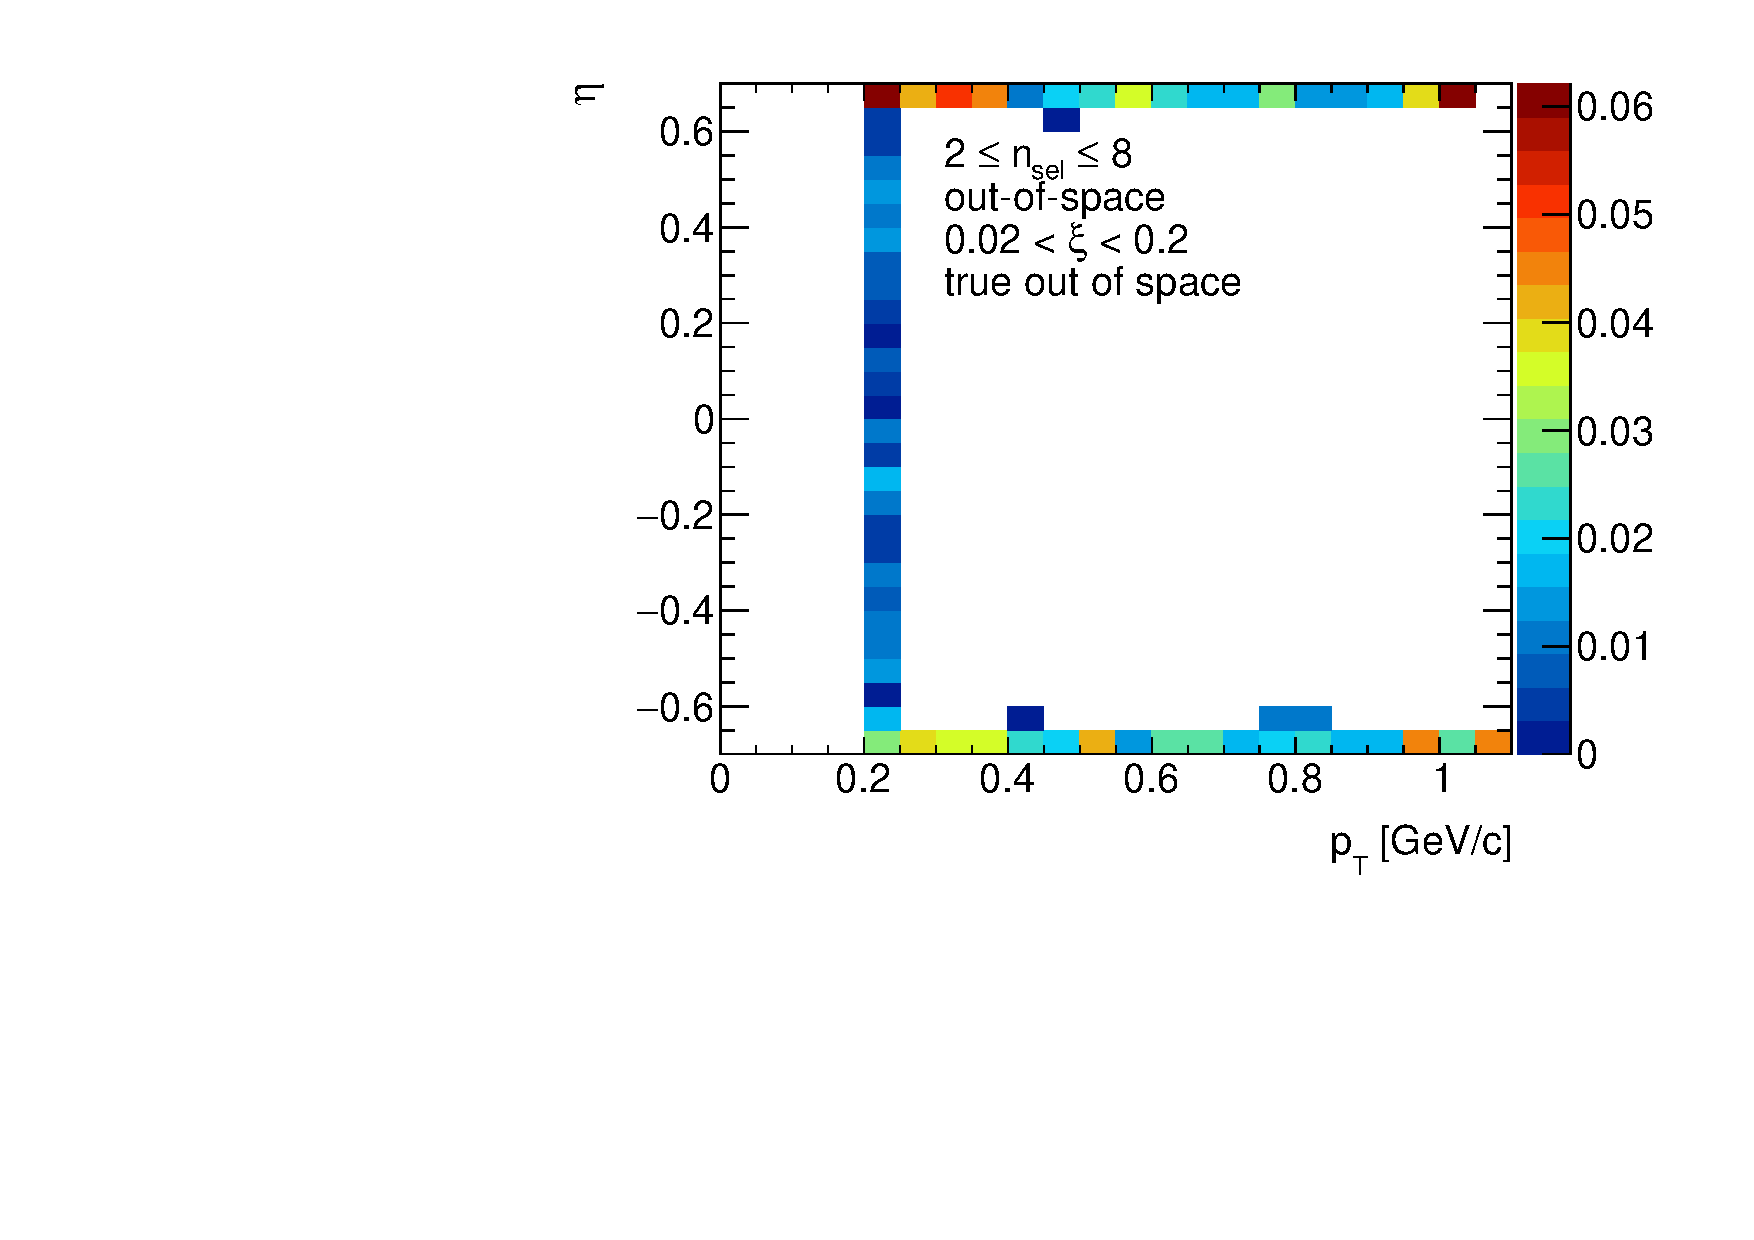
\includegraphics[width=0.49\textwidth, page=1]{chapters/chrgSTAR/img/OKR/outOfSpace.pdf}
	\includegraphics[width=0.49\textwidth, page=2]{chapters/chrgSTAR/img/OKR/outOfSpace.pdf}
	\caption{(left) Fraction of selected tracks migrating from outside of the kinematic range to the signal region and (right) fraction of particles for which the corresponding reconstructed track is outside the kinematic range of the measurement.}
	\label{fig:okr}
\end{figure}
\FloatBarrier